\newpage\chapter{Introduzione alla farmacologia}

\section{Definizioni generali}

\begin{description}

\item[Farmacologia] lo studio di sostanze che interagiscono con gli esseri vivnti con processi chimici, con molecole regolatrici e attraverso l'attivazione ol'inibizione di normali processi organici.

\item[Farmacologia medica] scienza che si occupa delle sostanze utilizzate per prevenire, diagnosticare e trattale le malattie

\item[Tossicologia] branca della farmacologia che si occupa degli effetti dannosi delle sostanze chimiche sui viventi

\item[Farmacogenomica] studio delle variazioni genetiche che causano differenze individuali nella risposta ai farmaci

\item[Farmaco] qualsiasi sostanza in grado di indurre, attraverso le sue azioni chimiche, modifiche di funzioni biologiche


\item[Recettore] molecola biologica che svolge un ruolo regolatorio.

\end{description}

\begin{tikzpicture}
	\Tree
	[.{Farmaco agisce}
		[.{sui recettori}
			{come agonista (attivatore)}
			{come antagonista (inibitore)}
		]
		[.{non mediata\\ da recettori}
			{agenti osmotici\\(mannitolo nei tubuli)}
			{interazione chimica diretta\\(antiacidi)}
		]
		[.{con altri farmaci}
			{come agonista o\\ antagonista chimico}
		]
	]
\end{tikzpicture}

\begin{tikzpicture}
	\Tree
	[.{Fisicamente è}
		{solido (aspirina, atropina...)}
		{liquido (nicotina, etanolo...)}
		{gas (protossido d'azoto)}
	]
\end{tikzpicture}

\begin{tikzpicture}
	\Tree
	[.{Composto da}
		carboidrati
		proteine
		lipidi
	]
\end{tikzpicture}

Dimensione da 7pm (litio) a 59000pm (alteplase) ma usualmente compreso da 100 a 1000pm.

\begin{description}

\item[Farmacodinamica] Definisce le azioni di un farmaco sull'organismo e le relazioni tra concentrazione e effetto.

\item[Farmacocinetica] Definisce le azioni dell'organismo sul farmaco e le relazioni tra dose e concentrazione, l'assorbimento, la distribuzione e l'eliminazione del farmaco

\item[Molecola effettrice/effettore] molecola che attiva la modifica funzionare finale. Può essere parte del recettore o una molecola separata.
\end{description}

Un farmaco (F) agisce su un recettore R attivando (*) un effettore (E) o passando per una molecola accoppiante (G) secondo una di queste tappe

\begin{eqnarray*}
F + R \longrightarrow FR + E \longrightarrow FRE^* \longrightarrow\text{effetto}\\
F + R \longrightarrow FR + E \longrightarrow E^* \longrightarrow\text{effetto} \\
F + R \longrightarrow FR + G \longrightarrow G^* + E \longrightarrow E^*  \longrightarrow\text{effetto}
\end{eqnarray*}

L'inibizione del metabolismo di un attivatore endogeno porta a \upa attivatore e quindi \upa effetto.

\begin{tikzpicture}
	\Tree
	[.{Interazione\\ farmaco\\ recettore}
		[.agonista
			{si lega al sito di legame e\\ attiva la funzione dell'agonista}
		]
		[.antagonista
			{si lega al sito di legame\\ impedendo la funzione dell'agonista}
		]
		[.{allosterico\\(su altro sito)}
			[.attivatore
				{aumenta la funzione dell'agonista}
			]
			[.inibitore
				{diminuisce la funzione dell'agonista}
			]
		]
	]
\end{tikzpicture}

Un recettore R senza agonisti vive normalmente in un equilibro fra la sua forma inattivata $R_I$ preferenziale e la sua forma attivata $R_A$. Quindi, anche senza agonista ha una sua attività di base detta \textbf{attività costitutiva}.

Un farmaco agonista sposta l'equilibrio verso $R_A$

\begin{eqnarray*}
\schemestart $R_I$\arrow{<<->}$R_A$ \schemestop \\
\schemestart $R_I + F$\arrow{<->>}$R_A + F$ \schemestop
\end{eqnarray*}

\begin{description}
\item[Agonisti pieni] quei farmaci che danno viraggio quasi completo di $R$ nella forma $R_A$
\item[Agonisti parziali] non stabilizzano la forma $R_A$ in modo completo. Questi, se presente un agonista pieno, si comportano da antagonisti nei confronti di quello pieno.
\item[Antagonista (neutro)] farmaco che blocca l'accesso al recettore prevenendone l'effetto ma ininfluente sull'equilibrio dello stato $R_I$
\item[Agonista inverso]farmaco che stabilizza lo stato $R_I$ diminuendo l'attività costitutiva del recettore
\end{description}

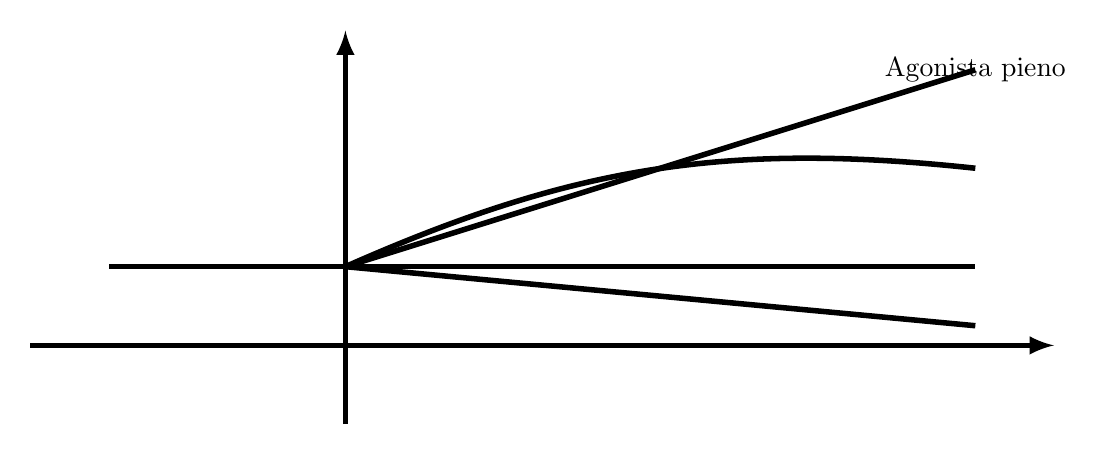
\begin{tikzpicture}
	\tikzstyle{none}=[inner sep=0pt]
	\tikzstyle{arrow1}=[-latex,draw,line width=2.000]
	\tikzstyle{simple}=[-,draw,line width=2.000]
		\node [style=none] (0) at (0, 4) {};
		\node [style=none] (1) at (9, -0) {};
		\node [style=none] (2) at (0, -1) {};
		\node [style=none] (3) at (-4, -0) {};
		\node [style=none] (4) at (-3, 1) {};
		\node [style=none] (5) at (0, 1) {};
		\node [style=none] (6) at (8, 3.5) {Agonista pieno};
		\node [style=none] (7) at (8, 2.25) {};
		\node [style=none] (8) at (8, 1) {};
		\node [style=none] (9) at (8, 0.25) {};

		\draw [style=arrow1] (3.center) to (1.center);
		\draw [style=arrow1, in=-90, out=90, looseness=1.00] (2.center) to (0.center);
		\draw [style=simple] (4.center) to (5.center);
		\draw [style=simple] (5.center) to (6.center);
		\draw [style=simple, bend left=15, looseness=1.00] (5.center) to (7.center);
		\draw [style=simple] (5.center) to (8.center);
		\draw [style=simple] (5.center) to (9.center);

\end{tikzpicture}

\begin{tikzpicture}
	\tikzset{level 3/.style={level distance=130pt}}
	\Tree
	[.{Meccanismo di diffusione}
		[.{verso il sito}
			[.{acquosa via}
				citosol
				{spazio interstiziale}
				{giunzioni serrate}
			]
			trasportatori
			endocitosi
			esocitosi
		]
		[.{fuori dal sito}
			[.{ABC\\(ATP binding cassette}
				{MPR\\(nel cervello, testicoli)}
				{MDR1\\(multidrug resistence proteine\\ nelle neoplasie)}
			]
		]
	]
\end{tikzpicture}

\begin{description}
\item[Legge di Fick]
$$ \Phi_{n.mol/s} = \Delta C \cdot \frac{S\cdot C_p}{d} \qquad\text{dove}$$

$\Delta C = C_1 - C_2$ differenza di concentrazione con $C_1 > C_2$\newline
$S$ area di diffusione\newline
$d$ spessore della via di diffusione\newline
$C_p$ coefficiente di diffusione

\item[Acido debole] molecola neutra che può reversibilmente dissociarsi in un anione 

$$\ce{HA <-> A- + H+}$$

\item[Base debole] molecola neutra che può reversibilmente formare un catione

$$\ce{BH+ <-> B + H+}$$

Poichè la diffusione lipidica è ostacolata dalla ionizzazione allora un acido debole ha diffusione lipidica in forma protonata mentre la base debole ha diffusione lipidica nella forma non protonata.

\end{description}

\section{Eq. di Hasselback}

Definisce il rapporto tra forma protonata e non sulla base della costante di dissociazione \ce{pK_a} della sostanza e il \ce{pH} dell'ambiente ove il \ce{pK_a} è il \ce{pH} ove \ce{[HA] = [A-]} e tale che

$$\log\frac{\ce{[HA]}}{\ce{[A^-]}} = \ce{pK_a} - \ce{pH}$$

che si applica sia alle basi che agli acidi deboli. Per cui a $\ce{pH} > \ce{pK_a}$ si avrà che quella più rappresentata è la forma deprotonata ossia quella lipofilica per le basi deboli mentre a $\ce{pH} < \ce{pK_a}$ quella più rappresentata sarà quella protonata ossia la forma lipofilica per gli acidi deboli.



